%! Author = Omar Iskandarani
%! Date = 2025-06-13

% === Metadata ===
\newcommand{\papertitle}{Kairos Moments and Topological Transitions in VAM}
\newcommand{\paperauthor}{Omar Iskandarani}
\newcommand{\paperaffil}{Independent Researcher, Groningen, The Netherlands}
\newcommand{\paperdoi}{10.5281/zenodo.15566319}
\newcommand{\paperorcid}{0009-0006-1686-3961}

\ifdefined\standalonechapter\else
% Standalone mode
\documentclass[12pt]{article}
\usepackage[a4paper, margin=2cm]{geometry}
\usepackage{ifthen} % we can use it safely now
\usepackage{import}
\usepackage{subfiles}
\usepackage{hyperref}
\usepackage{graphicx}
\usepackage{amsmath, amssymb, physics}
\usepackage{siunitx}
\usepackage{tikz}
\usepackage{booktabs}
\usepackage{caption}
\usepackage{array, tabularx}
\usepackage{listings}
\usepackage{bookmark}
\usepackage{newtxtext,newtxmath}
\usepackage[scaled=0.95]{inconsolata}
\usepackage{mathrsfs}
% vamappendixsetup.sty

\newcommand{\titlepageOpen}{
  \begin{titlepage}
    \thispagestyle{empty}
    \centering
    \vspace*{2cm}
    {\Huge\bfseries \appendixtitle \par}
    \vspace{1cm}
    {\Large\itshape \appendixauthor \par}
    \vspace{0.5cm}
    {\small \appendixaffil \par}
    ORCID: \href{https://orcid.org/\appendixorcid}{\appendixorcid} \\
    DOI: \href{https://doi.org/\appendixdoi}{\appendixdoi} \\
    \vspace{0.5cm}
    {\large \today \par}
    \vspace{1cm}
}

\newcommand{\titlepageClose}{
  \vfill
  \end{titlepage}
}

\begin{document}

    % === Title page ===
    \titlepageOpen

    \begin{abstract}
        This appendix formalizes the notion of \textit{Kairos Moments} within the Vortex \AE{}ther Model (VAM) as topological or energetic bifurcations in the evolution of the vortex field. We define the mathematical and physical criteria that trigger such irreversible transitions, including vorticity singularities, helicity loss, and discontinuities in swirl-based clock rates. These events segment continuous æther-time into distinct epochs and provide a mechanism for encoding structural memory within the æther.
    \end{abstract}



    \titlepageClose
    \fi

% ============= Begin of content ============
    \section{\papertitle}

    \subsection*{Overview}
    In the Vortex \AE{}ther Model (VAM), time is structured into distinct modes:
    \begin{itemize}
        \item \textbf{Aith\={e}r-Time} (\( \mathcal{N} \)): universal causal background
        \item \textbf{Chronos-Time} (\( \tau \)): proper time along macroscopic trajectories
        \item \textbf{Swirl Clock} (\( S(t) \)): local clock rate modulated by vorticity energy
        \item \textbf{Vortex Proper Time} (\( T_v \)): time along rotating core structures
        \item \textbf{Kairos Moment} (\( \kappa \)): irreversible topological or energetic bifurcation
    \end{itemize}
    Among these, \( \kappa \) marks critical transition points where smooth time evolution in \( \mathcal{N} \) or \( \tau \) cannot be maintained.

    \subsection{Definition of a Kairos Moment}
    A \textit{Kairos Moment} \( \kappa \) is defined as a non-analytic point in the evolution of the vortex æther field, typically accompanied by a discontinuity in the temporal or topological structure:
    \begin{equation}
        \lim_{\epsilon \to 0} \left( \frac{d\vec{\omega}}{dt} \right)_{t = \kappa - \epsilon}
        \neq
        \left( \frac{d\vec{\omega}}{dt} \right)_{t = \kappa + \epsilon}.
    \end{equation}

    Such moments correspond to irreversible events like:
    \begin{itemize}
        \item vortex reconnection,
        \item knot topological transitions (\( \Delta Lk \in \mathbb{Z} \)),
        \item swirl energy overloads,
        \item swirl clock rate rupture.
    \end{itemize}


    \begin{figure}[h]
        \centering
        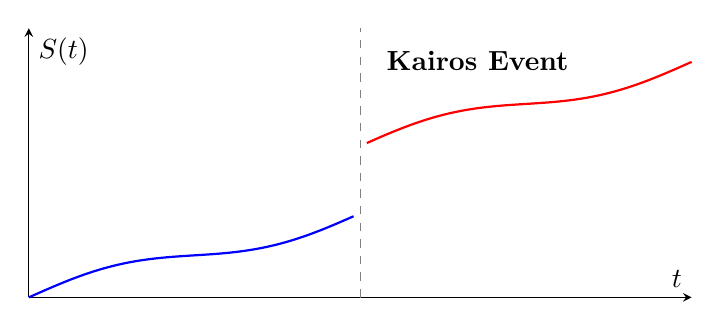
\begin{tikzpicture}

            \begin{axis}[
            axis lines=middle,
            xlabel={$t$},
            ylabel={$S(t)$},
            xtick=\empty,
            ytick=\empty,
            xmin=0, xmax=10,
            ymin=0, ymax=8,
            width=10cm,
            height=5cm,
            samples=100,
            domain=0:10,
            smooth,
            clip=false
            ]

% Swirl clock function before jump
            \addplot[thick, blue, domain=0:4.9] {0.5*x + 0.3*sin(deg(2*pi*x/5))};
% After jump
            \addplot[thick, red, domain=5.1:10] {0.5*x + 0.3*sin(deg(2*pi*x/5)) + 2};

% Kairos event line
            \addplot[dashed, gray] coordinates {(5,0) (5,8)};

            \end{axis}

% Kairos label above the dashed line
            \node at (5.7,3.0) {\textbf{Kairos Event}};

        \end{tikzpicture}
        \caption{Swirl clock bifurcation at $t = t_c$: a topological reconnection causes a discrete phase shift in $S(t)$.}
    \end{figure}


    \subsection{Trigger Conditions for Kairos Transitions}
\begin{eqbox}
    \begin{table}[H]
        \centering
        \footnotesize
        \renewcommand{\arraystretch}{1.4}
        \begin{tabular}{|c|l|l|}
            \hline
            \textbf{Type} & \textbf{Trigger Condition} & \textbf{Physical Interpretation} \\
            \hline
            \textbf{1. Vorticity Gradient Singularity} &
            $|\nabla \vec{\omega}| \geq \dfrac{C_e}{r_c^2}$ &
            Core rupture or instability onset \\
            \textbf{2. Helicity Discontinuity} &
            $\Delta H \neq 0$, $\Delta Lk \in \mathbb{Z}$ &
            Knottedness transition \\
            \textbf{3. Energy Threshold Exceeded} &
            $U_{\text{swirl}} > U_{\text{max}} = \frac{1}{2} \rho_{\text{\ae}} C_e^2$ &
            Collapse from over-rotation \\
            \textbf{4. Vortex Collision} &
            $\vec{\omega}_1 \cdot \vec{\omega}_2 < 0$, at $|\vec{r}_1 - \vec{r}_2| < \delta r_c$ &
            Reconnection or annihilation \\
            \textbf{5. Swirl Clock Discontinuity} &
            $\left.\frac{dS}{dt}\right|_{t = \kappa^-} \neq \left.\frac{dS}{dt}\right|_{t = \kappa^+}$ &
            Local time rupture in vortex cores \\
            & & \\
            \hline
        \end{tabular}
        \caption{Trigger conditions for Kairos transitions in the vortex æther field.}\label{tab:table}
    \end{table}
\end{eqbox}

    \subsection{Energetic Criterion from Swirl Potential}
    Kairos events are energetically triggered when local swirl energy exceeds the maximum sustainable value in the æther medium:
    \begin{equation}
        U_{\text{swirl}} = \frac{1}{2} \rho_{\text{\ae}} |\vec{\omega}|^2,
        \quad
        U_{\text{max}} = \frac{1}{2} \rho_{\text{\ae}} C_e^2.
    \end{equation}
    Hence, the condition:
    \[
        U_{\text{swirl}} > U_{\text{max}}
    \]
    triggers structural realignment, swirl rupture, or reconnection.

    \subsection{Helicity and Knot Transitions}
    The total helicity \( H \) of a vortex system is given by:
    \begin{equation}
        H = \int \vec{v} \cdot \vec{\omega} \, dV,
    \end{equation}
    which is conserved under smooth evolution. However, when:
    \[
        \Delta H = H_{\text{after}} - H_{\text{before}} \neq 0,
    \]
    a topological transformation has occurred, such as knot reconnection or linking number jump (\( \Delta Lk \in \mathbb{Z} \)) — a definitive marker of \( \kappa \).

    \subsection{Temporal Discontinuity in Swirl Clocks}
    Swirl clocks \( S(t) \) track local time using vorticity-based rates. A Kairos moment induces a discontinuity in the swirl time derivative:
    \begin{equation}
        \lim_{\epsilon \to 0} \left[ \frac{dS}{dt}(t = \kappa - \epsilon) \right]
        \neq
        \left[ \frac{dS}{dt}(t = \kappa + \epsilon) \right].
    \end{equation}
    This represents an irreversible reconfiguration of the internal clock rate, isolating vortex epochs before and after \( \kappa \).

    \subsection{Interpretation Across Time Modes}

    \begin{table}[H]
        \centering
        \renewcommand{\arraystretch}{1.3}
        \begin{tabular}{|c|c|p{9cm}|}
            \hline
            \textbf{Time Mode} & \textbf{Symbol} & \textbf{Effect at Kairos Moment} \\
            \hline
            Aithēr-Time & \( \mathcal{N} \) & Globally continuous, but re-indexed at \(\kappa\) \\
            Chronos-Time & \( \tau \) & Broken derivative continuity (\( d\tau/dt \) jump) \\
            Swirl Clock & \( S(t) \) & Discontinuous rate: \( \Delta \left(\frac{dS}{dt}\right) \neq 0 \) \\
            Vortex Proper Time & \( T_v \) & Reset or bifurcation of local vortex clock phase \\
            Kairos Marker & \( \kappa \) & Singular time point; cannot be evolved through \\
            \hline
        \end{tabular}
        \caption{Temporal ontology response to a Kairos transition.}
    \end{table}


    \subsection{Experimental Analogy}
    An accessible analogy to Kairos transitions exists in superfluid helium (\(^4\)He), where vortex reconnections are captured by tracer
    particles and Kelvin waves~\cite{bewley2006} These observations reveal the discontinuous evolution of topological structures, paralleling the role of \( \kappa \) in VAM.

    \subsection*{Conclusion}
    Kairos Moments \( \kappa \) encode the breakdown of smooth time evolution in the Vortex Æther Model. They delineate epochs of distinct
    topological and energetic configurations, demarcate irreversible transitions, and formalize events beyond the classical conservation paradigm. These singularities lie at the intersection of topology, dynamics, and temporality — and serve as central markers in vortex chronology. While the concept of Kairos Moments is novel to the Vortex Æther Model, it draws inspiration from quantized vortex reconnections observed in superfluid helium~\cite{bewley2006}, helicity transitions in classical fluid dynamics~\cite{moffatt1969}, and non-analytic behavior in phase transitions~\cite{landau1959}.







% === Bibliography (only for standalone) ===
    \ifdefined\standalonechapter
    % Being imported from main.tex — do nothing
    \else
    \bibliographystyle{unsrt}
    \bibliography{../../references}
    \end{document}
    \fi